\documentclass[11pt,letterpaper]{article}
\usepackage[utf8]{inputenc}
\usepackage{amsmath}
\usepackage{authblk}
\usepackage{amsfonts}
\usepackage{amssymb}
\usepackage{graphicx, caption}
\usepackage[left=1in,right=1in,top=1in,bottom=1in]{geometry}
\usepackage{fancyhdr}
\pagestyle{fancy}
\usepackage{adforn}
\usepackage{subcaption}
\usepackage{placeins}

\begin{document}
\title{Long Range Resonant Inductive\\Wireless Power Transfer White Paper}
\author{\adforn{21}\\\vspace{12pt}\textsc{Cole Nielsen}}
\date{}
\affil[]{\textsc{EE 4161W} }
\maketitle
\vskip-2ex
\noindent\hrulefill
\FloatBarrier
\begin{abstract}
\noindent Wireless power transfer (WPT) has the potential to revolutionize how electronics are powered by removing the need for cable-based power solutions. Resonant-inductive technology current represents an option for medium to long range power transfer, perhaps viable to power mobile electronics. Transmitter arrays featuring this technology could be built in arrays to power devices within range with total mobility. Practical considerations regarding mobility of people within the transmitter area coupled with physical limits however suggest it may not be possible to implement such a technology as suggested. It was found that to power a cell phone at one meter with no obstruction to the mobility of the user, a transmitting system using this technology would have as low as 0.25\% efficiency. Further considerations, being cost of installation and undesirable electromagnetic interaction inherent from the technology suggest its non-viability for an actual mobile device wireless power system. Overall resonant-inductive WPT is not recommended for powering of mobile devices due to immense design challenges, rather an alternative technology such as beam forming of radio waves is recommended.  
\end{abstract}
\noindent\hrulefill
\section*{\large Introduction}
\noindent The abundance of mobile electronics today has placed continual demand on manufacturers to increase device battery life. With a slow rate of increase attributed to the energy density of tradition battery storage like LiPo cells, the usage of alternative technologies to power today's devices is becoming more attractive. One such technology is resonant-inductive wireless power transfer. Before going into detail on the resonant aspect, a quick primer on inductive wireless power transfer (WPT) will be presented. The basic principle here is the idea of magnetic induction, which begins by inducing a changing magnetic field in a coil of wire with a alternating current. If one places a second coil so that the first coil's field passes through it (that is, they \textit{couple}), a voltage will be induced across that coil. It becomes interesting when you connect a load (think a resistor or some device) to the second coil (more properly the \textit{secondary} coil). A current will be induced by the potential and power will be dissipated! This means power can be transferred to a load- perhaps a phone- wirelessly if the coils are physically separate. This is therefore the solution to the battery problem. Instead of relying on battery life, one could use coils built into the surrounding environment (house, office, streets) to transfer power magnetically to your mobile device on demand. Figure \ref{fig_sim} demonstrates this idea.
\begin{figure}[!t]
	\centering
	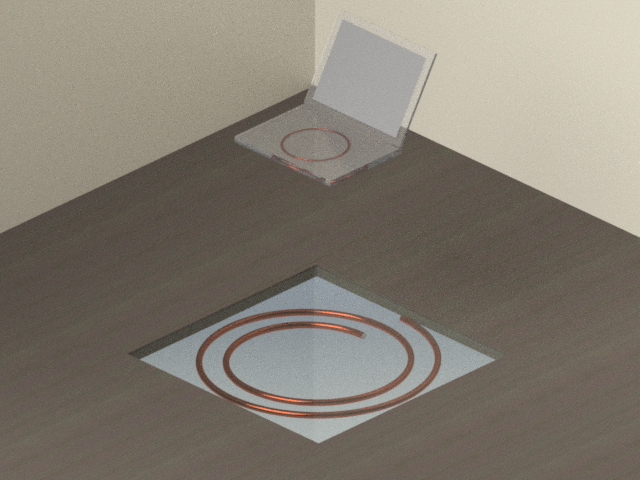
\includegraphics[width=0.7\linewidth]{Image.png}\\
	\captionsetup{width=.7\linewidth}
	\caption{\small Visualization of a hypothetical resonant inductively coupled WPT system. The picture shows a large transmitter coil built into the floor of a room that would emit power via a oscillating magnetic field. A computer, shown hovering above the transmitter would also contain a coil as shown that would couple to the transmitted magnetic flux and absorb transmitted power. Note the receiving coil is much smaller than the transmitter. A large transmitter coil is needed in order to allow for reasonable coupling to the receiving device over a large number of positions. A challenge associated with this is a small portion of the transmitters flux passes through a given receiver. Therefore the transmitter requires a very high Q to ensure energy of the flux not coupled to the receiver is not lost, but stored to be later absorbed by the receiver.}
	\label{fig_sim}
\end{figure}
 The primary issue that has prevented this idea from being implemented is the physical limitations of coil coupling. Coil coupling describes quantitatively how a current in the first coil (\textit{primary}) induces voltages in the secondary. For WPT is it easier to think of it in terms of the proportion of the magnetic flux from the first coil that makes it through the secondary coil. As fields tend to decrease as the inverse of distance squared, it is easy to imagine that coupling decreases fast with distance. This means the amount of power that can be transfered over a distance inductively falls rapidly- a problem. \\\par 
 \FloatBarrier
\noindent A solution to this crux is resonance \cite{duong}. The basis of this method is to increase the amount of magnetic flux that reaches the secondary coil. This can be traditionally by increasing the source current, but practically this is hard as huge currents are needed, which implies low driver efficiency. This is achieved "resonantly" by in effect using repeater coils to relay magnetic fields from a transmit to receive coil. These coils are typically constructed out of a extremely low resistance conductor with a capacitor connected at its ends, forming a LC resonator with high Q. These coils are tuned to resonate at the frequency which drives the primary (transmitter) coil. The effect this has is repeater coils will store most of the energy that couple to them, resulting in huge currents which flow through them and accordingly induction of strong magnetics fields locally. If fed by the primary coil, these coils can produce strong magnetics fields at a distance which exceed that normally produced just by the primary coil. This can therefore by used to induce stronger magnetic fields in some receiving device at a distance, and thus deliver more power to it. This is the basic principle of resonant-inductive WPT.\\\par 
\noindent The question then stands if resonant-inductive WPT can be implemented in a practical manner to power typical mobile devices with sufficiency power, reliability and economic feasibility. This paper seeks to address these questions, looking at typical usage scenarios of mobile devices and according needs for WPT system, technical challenges and requirements and economics consideration. From this a conclusion will be formed on the viability of this technology to power devices.
\section*{Technology and Feasibility}
Assuming a resonant-inductive power transmitter system is built into the ground of an environment, it is reasonable to assume the distance a device to ground would be within the height of a person. This is perhaps 2 meters. The size and power of typical devices needs to be considered. (1) A typical laptop ranges from 11-17" diagonally, consumes 5-20W, (2) a tablet is 7-12" diagonally, consumes 2-5W, and (3) a cell phones is 5-6" diagonal, consumes 0-2W. The receive coil thus must fit in these respective size constraints and deliver the listed power. To begin our analysis, the average magnetic field needed to pass through a phone to power it will be estimated. This is simple to approximate with the Biot-Savart law and Faraday's law for a single loop receiver. The result of such a derivation is:
\begin{equation}
	B_{n,RMS} = \sqrt{\frac{\sqrt{2}\mu_0 P_{Load}}{2\pi f r A }}
\end{equation}  
Namely P$_{Load}$ is the device power, f is frequency of oscillation, and r and A are the receive coil radius and area (governed by device size). An interesting question is what frequency should be used for the system; equation 1 shows there is a inverse root proportionality for needed B field to frequency. Therefore $f$ should be made large to reduce the field, but not to the extent where dielectric heating is a risk to people. $f$ should also be chosen to hold compliance with the FCC. ISM bands are a natural choice, with the 6.78MHz, 13.56MHz and 27.12MHZ bands representing a good choice. An estimate now can be made for the cell phone field, assuming the previous estimates for size, power and now an assumption of 13.56MHz operation. A quick calculation yields an estimate of B = 20$\mu$T RMS normal field to the phone. \\\par 

\noindent For reasonable mobility of the user, repeater coils must not be too close to user, so perhaps a constraint for this would be one meter (likely embedded in the room floor, walls, ceiling, table tops). The question now is the field required at the repeater coil to provide a 20$\mu$T field at 1 meter. Again applying the Biot-Savart law again it is found: 
\begin{equation}
	B_Z = B_0 \frac{(Z^2 + R^2)^\frac{3}{2}}{R^3}
\end{equation}
Where Z is the coil separation, R is the repeater coil diameter, and B$_0$ is the 20$\mu$T field required at the phone B$_Z$ is the field at the repeater coil. It is arguable that the repeater coil should be made large for cost reasons as one would expect it be cheaper to install and manufacture a system requiring fewer parts (assuming many repeater coils are needed in a system installation). Perhaps a diameter of 12" would be reasonable, to yield 1 repeater per sq. ft. in a array. This leads to the field at the repeater being B = 820$\mu$T. Upon first glance, this may not seem large, however this corresponds to a current of 200A in the repeater coil for one 12" turn. Ohmic loss is given by $I^2R$, and if the repeater is assumed to have a very forgiving 10m$\Omega$ series resistance, this corresponds to a 400W loss to deliver 1W to a phone ($\frac{1}{4}$\% efficiency). This issue brings into question the viability of resonant-inductive WPT, as practically the repeater coils should not be close to the device user and device.\\\par 

\noindent To consider this technology from an economic standpoint, the cost to integrate resonant-inductive WPT throughout an entire room should be considered. The main consideration here is the cost for the coil driver electronics, transmitter and repeater coils. To maintain even power coverage throughout a room, an array of many transmitter coils and repeater are needed. For easy installation, one transmitter coil system per 2 foot by 2 foot area is possible, perhaps at a cost of \$100 per transmitter system to install. This works out to \$25 per square foot, likely outside of the reach for individual consumers as cost per 1000 sq ft would be \$25000, however feasible for spaces shared by many users such as an office space. \\\par 

\noindent A few other considerations of this technology are its biological effects and interaction with objects in its presence. One primary concern is losses from Eddy currents induced in metallic objects within the range of the WPT system. A solution would be to not allow large metallic objects within the WPT systems influence, however this does not seem practical in any regard. There is also a question of electromagnetic interference due to the large fields generated by the coils. It is possible that the strong fields generated can cause devices in range to malfunction as a results of energy coupling into circuits. A last concern is biological impacts due to absorption of electromagnetic fields. This is perhaps not an issue at the relatively low frequency suggested in this report as dielectric heating is minimal in the low MHz region of the radio spectrum. However there may be other biological effects that are repercussions of the high strength and relatively high frequencies fields generated that are not yet totally understood or known. 

\section*{Conclusion}
The feasibility of a resonant-inductive wireless power transfer system was analyzed for medium range distance (1-2m) to power mobile devices in a practical manner. Practical was interpreted as providing no inconvenience (mainly mobility) to the user of the device compared to traditional means. After analysis, it was found that this technology is not feasible for the described application. This stems from inherently low coupling needed to permit reasonable mobility to a device user, which massively degrades efficiency to levels as low as 0.25\% to deliver 1W to a cell phone. Although this system may be effective from a cost standpoint, it is probably unlikely that enough momentum could be gathered to be integrated into common electronics, or to get enough installed square footage of transmitters. Lastly, interaction of the required magnetic fields with objects in it has been deemed unacceptable as there is risk for induction of large Eddy currents (thus heating) in metallic devices, as well as interference with electronic devices.
\begin{thebibliography}{1}
	
	\bibitem{massa}
	1. A. Massa, G. Oliveri, F. Viani and P. Rocca, "Array Designs for Long-Distance Wireless Power Transmission: State-of-the-Art and Innovative Solutions," in Proceedings of the IEEE, vol. 101, no. 6, pp. 1464-1481, June 2013.
	\bibitem{duong}
	T. P. Duong and J. W. Lee, "Experimental Results of High-Efficiency Resonant Coupling Wireless Power Transfer Using a Variable Coupling Method," in IEEE Microwave and Wireless Components Letters, vol. 21, no. 8, pp. 442-444, Aug. 2011.
	\bibitem{choi}
	B. H. Choi, E. S. Lee, J. H. Kim and C. T. Rim, "7m-off- long-distance extremely loosely coupled inductive power transfer systems using dipole coils," 2014 IEEE Energy Conversion Congress and Exposition (ECCE), Pittsburgh, PA, 2014, pp. 858-563.

\end{thebibliography}





\end{document}